\documentclass{style/CRPITStyle}
\usepackage{epsfig}   % Packages to use if you wish
\usepackage{lscape}   %
\usepackage[authoryear]{natbib}
\renewcommand{\cite}{\citep}
\pagestyle{empty}
\thispagestyle{empty}
\hyphenation{roddick}

\begin{document}

\title{Software Development Life Cycles: History and Future}
\author{David Barnett}
\affiliation{School of Engineering and Computer Science \\
Victoria University of Wellington, \\
PO Box 600, Wellington, 6140 \\
Email:~{\tt barentdavi@myvuw.ac.nz}}

\maketitle

\begin{abstract}
    % TODO
    Abstract goes here
\end{abstract}

\vspace{.1in}

\noindent {\em Keywords:} Software Process Models

\vspace{.1in}

% \section{Introduction}
% TODO
% thesis statement

\section{Importance of using process models}
% Q: describe the importance of using process models to guide software development

% why we need process modeling
Fail to plan, is a plan to fail. 
As software has increased in complexity and scale of projects increase it
became more apparent that software should be managed and planned differently it was
described as a \emph{Software crisis} \cite{nato:1969}.
``We believe that the only way ahead lies through the steady development of the best existing 
techniques'' \cite{nato:1969} Gill's comments on how to move forward from the
\emph{Software Crisis} which describes a need for more of an engineering approach to software development.
One such endeavour is process modelling.
A process model is a model of how to setup a project with a set of tasks,
such as requirements acquisition or construction, of a similar nature that together form 
the scaffolding of a plan of how to approach to build a project.

\vspace{.1in} % are we allowed to do this?

By using the appropriate process model software development can be guided
through the many stages of creating software with an over-arching idea of how it
should be done. This can range from having static requirements and working
linearly through the development cycle to changing the requirements from week to
week. With the right processing model the software will have the correct tools
to handle what was expected to happen through out the process and give a guide
through the unexpected.

% add more on why it is important and how it guides

\section{Review of Process Models}

% TODO: this needs some reworking
Over the years many process models have been proposed and many variations have
been used and reported one. The process models that will be discussed in this
review is: Waterfall, V-Model, Spiral Model, Iterative and Incremental Development and
Extreme programming.

% --- 5 Model Section ---
% Q: provide a systematic review of process models that have been proposed so far,
% Q: compare and contract 5 selected distinct process models for software development
% Q: identify central themes that have been considered important for evolving process models
\subsection{Waterfall} % sequential
% theme: sequential
% strengths: requirements up front, easy
% Goals: a model of how to make successful large software
% Strengths: easy, clear steps and deliverables
% compare: ??
% contrast: ??
% note: Need a counter source, "Enough with Life cycle?"

% should include an overview & theme of the model
The Waterfall model was proposed in 1970 by Dr. Winston Royce \cite{royce:1970:waterfall} 
with a focus on meeting requirements.
He proposed it as a method to be a guide of steps and processes that together
help to make a larger software project succeed. 
The principle idea behind the Waterfall model is that there are seven stages to
software development cycle and they are to be executed in a sequential order:

\begin{enumerate}
  \item System requirements
  \item Software requirements
  \item Analysis
  \item Design
  \item Coding
  \item Testing 
  \item Operations
\end{enumerate}

The end of each stage is a milestone of how the project is progressing and with some artifacts
that the next stage depends on, making them static for simplicity, and builds upon
them to deliver the next milestone till the product at the end of the process is
complete.

\begin{figure}[htb]
\fbox{\parbox[b]{.99\linewidth}{
\vskip 0.5cm
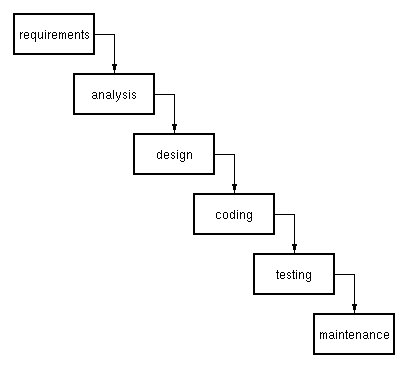
\includegraphics[width=0.45\textwidth]{figures/waterfall-model.png}
\vskip 0.5cm}}
\caption{\protect\label{waterfall}  Waterfall Model}
\end{figure}

Figure 1 shows the general form that Waterfall takes with its characteristic 
linearly moving between each stage with no movement back to previous stages of
development.

\vspace{.1in}

% main features of waterfall
The strength of this model lies in the assumptions that the requirements are
well thought out, any foreseeable problems has known solutions to complete the
software.
This lends the model to be more suitable for software projects that have well known
requirements and technology such as porting an application to another platform.
Waterfall also has the benefits of being an easy project to manage with its
clear milestones of development and equally easy for a new member or external
stakeholder to the team to understand the status of the project.

\vspace{.1in}

% covers the weakness of water fall
Conversely the strengths of the model also highlights the weaknesses of the model as
well.
One of the assumptions in the process model is that the requirements at the start of the project is
static and are still meet the clients needs that the project was started for.
Another factor to this weakness is that the model allows for only one delivery of the product to
the client at the end of the whole project, making a possible large time gap from requirements 
gathering with the client to the final delivery to the client which has the risk of not being 
what the client had in mind during the initial phases of the project.

\subsection{V-Model} % sequential, testing
% theme:
% Goals: to extends the existing Waterfall to include testing
% compare: Waterfall's steps
% contrast: Has testing involved in the 

% should include an overview & theme of the model
V-Model was proposed as a variation of the Waterfall model by Paul Rook in 1986
\cite{rook:1986:vmodel} with a testing focus.
The principle idea of the V-Model is to produce software in a linear fashion with
well known requirements and solved problems that has the need for extensive testing 
and verification of the system \cite{rook:1986:vmodel}.
The general workings of the V-Model are similar to the workings of Waterfall
with a few differences in testing.
Instead in V-Model the testing stage of the process model is expanded and added short loops,
the software is tested against the produced designs and requirements with
steps of verification and validations  that if failed will lead back to the design
stages or requirements respectfully.

\begin{figure}[htb]
\fbox{\parbox[b]{.99\linewidth}{
\vskip 0.5cm
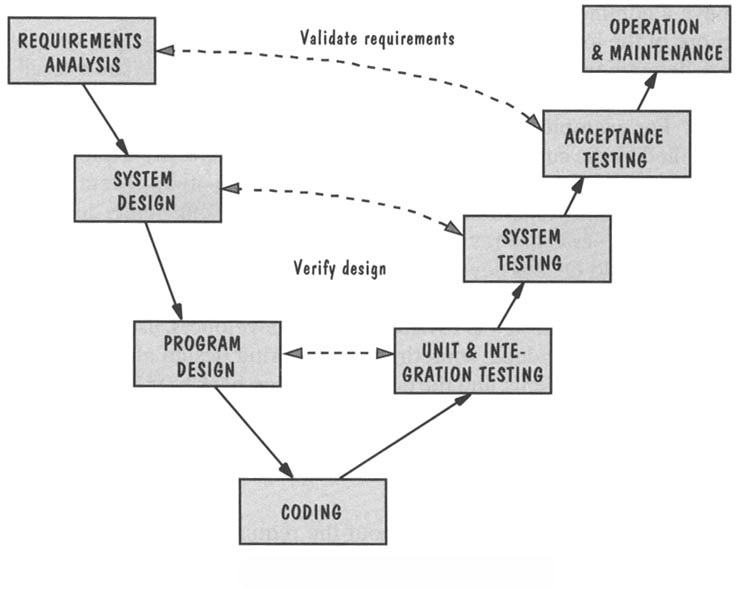
\includegraphics[width=0.45\textwidth]{figures/v-model.jpg}
\vskip 0.5cm}}
\caption{\protect\label{vmodel}  V-Model}
\end{figure}

Figure 2 shows a common interpretation of V-Model with its characteristic
building of requirements and designs to be tested against on the left side of
the model leading to the building of the software then moving up the right side
verifying and validating the software built against the specification built
earlier. Failure to meet leads back to the appropriate to re-visit building that
level of the design or the specification. Finally at the end releasing the
product to the client.

\vspace{.1in}

The strengths of the V-Model are built up upon Waterfall.
As with Waterfall, V-Model also is an easy to mange project with clear milestones
to each stage of development.
V-Model splits off from Waterfall with its focus
on verification and validation of the product.
Each artifact from the milestones are also used in the process again with either
being an artifact to test or to test against to verify and validate the product
moving forward. Failing to pass the test will lead back to the stage allowing to
fix a past mistake, recognising that it is hard to get it prefect the first time
round.
Through the testing the V-Model has the potential to produce an extensively well
tested product that meets a set of strict requirements such as traffic networks
or medical equipment \cite{advancements:2010:vmodel}.

\vspace{.1in}

% needs a cite in it somewhere
The shortcomings of V-Model as well is akin to Waterfalls.
V-Model relies upon the requirements are quite static but has slightly more
flexibility than Waterfall due to the addition of more extensive testing that introduced loops 
through the verification and validation processes of the product. 
The extensive testing is only truly beneficial given that the project needs to
be tested to such lengths, in situations that the end-product is used in safety
critical situations the testing will be a great asset but for other types of
projects that do not need a high level of verification and validation it would
be an expensive use of resources on an area for little benefits.
However this does not allow V-Model to be as flexible as iterative process models such as
Agile based models as V-Model still have a large time period between project
initiation and delivery. 
V-Model also suffers from the same fate of Waterfall in the fact that it only
delivers a single version of the product to the client. Which carries a risk of 
not meeting the clients needs, though it is indirectly managed through the validation testing.
This is an inherent risk of only delivering a single version at the end
of project common in sequential process models like V-Model and Waterfall.


\subsection{Spiral Model} % sequential / Iterative, testing, risk
% theme: sequential / iterative, risk
% compare:
% contrast:

The Spiral Model is a process model that Barry Boehm described in 1986 \cite{boehm:1988:spiral}.
The model has a mixture of ideas in it, the core idea of the model is to address risk management and analysis
which neither Waterfall or V-Model directly tackled.
Spiral model also shares some ideas from both Waterfall and V-Model with a sequential approach 
but also includes some iterative elements with producing multiple prototypes of the 
product over the course of the whole project but only delivers a single product
at the end of the development.
The rest of the process progresses linearly going through the software 
development cycle with the addition of steps to review and plan for
the next iteration of the prototype as well as identifying risks and
how to resolve them going forward.

\begin{figure}[htb]
\fbox{\parbox[b]{.99\linewidth}{
\vskip 0.5cm
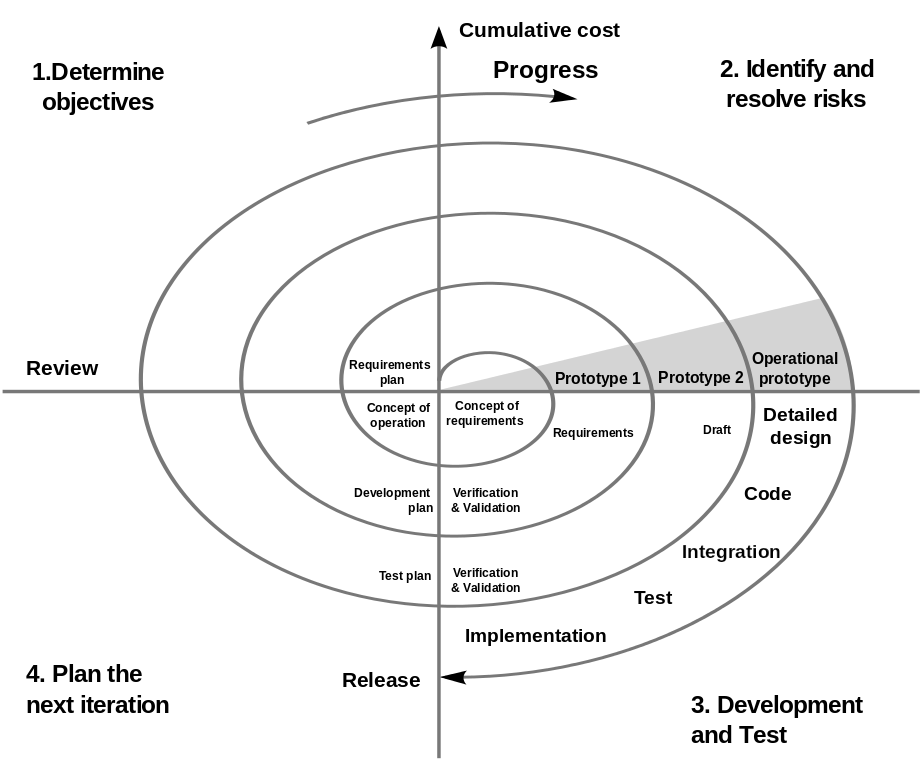
\includegraphics[width=0.45\textwidth]{figures/spiral-model.png}
\vskip 0.5cm}}
\caption{\protect\label{spiral}  Spiral Model}
\end{figure}

\vspace{.1in}

Figure 3 shows the general use of the Spiral Model, with some simplifications, 
with multiple cycles or iterations \cite{boehm:1988:spiral}.
Each cycle of the spiral starts with the identification of highest risk parts of the
final product to be developed in this iteration, shown as quadrant one in figure 3. 
This process also includes suggesting alternative ways to implement what
has been identified and
identifying the resource constraints for the cycle.
The next quadrant's goal is to handle risk analysis and resolving the identified
risk, allowing ``risk-driven subsetting of the spiral model steps allows the model 
to accommodate any appropriate mixture of a specification-oriented, 
prototype-oriented, simulation-oriented, automatic transformation-oriented, 
or other approach to software development'' \cite{boehm:1988:spiral}.
Which lends Spiral model to be very flexible with its application.
The third quadrant is the execution of the planning for the cycle with
development, testing and verification of the produced prototype form the
iteration. 
The final quadrant is to review the work that has been done including key
stakeholders in the review process.
% finish the overview of Spiral ^
% Done: 1, 2, ~3 

\vspace{.1in}

% Explicitly state Strengths + themes
The strength of the Spiral model comes from its ability to be
flexibility with how the project can be focused on a range of
different aspects such as specification or prototype.
Another strength is its ability to monitor and control through the whole process
of the development, which allows the project to explore solutions to problems
where in Waterfall or V-Model will be force to stick to the tried and true
methods instead of having the potential to innovate as spiral does.
With the inclusion of iterations Spiral has a large benefit of getting user and
client feedback during the development process to ensure the final product meets
the client's on important aspects such as user interface. This is a large
advantage above sequential models such as Waterfall that do not include any
explicit user interface iteration and refinement.

\vspace{.1in}

With the benefits and flexibility that the Spiral Model offers it comes at a
cost. 
One of them are the complexity to manage a project with Spiral, the process of
repeated iterations involve a considerable amount of overhead and repeated work
that is saved in Waterfall or V-Model. One such
problem is falling into the trap of running each cycle of the spiral as if it
was a miniature Waterfall.
The iteration are excellent for tracking the progress of the project but not all
projects benefits can be completed in parts and must be completed holistically
such as software supporting critical infrastructure where a sequential model
like V-Model is better suited.
Another cost of Spiral model is the need to have an expert of the risks that
will be needed to be identified and resolved which could cause a large strain on the
resources of the project than the benefits of mitigating the risks.

\subsection{Iterative and Incremental Development} % iterative, testing, risk
% theme: iterative, many deliverables
% goal: to build a working product every cycle and build upon it
% compare: Spiral
% contrast: Waterfall

\subsection{Extreme Programming} % iterative, testing, risk
% theme:
% compare:
% contrast:

\section{Possible evolutions of process models}
% Q: try to forecast how current process models may evolve in the future


\bibliographystyle{agsm}
\bibliography{essay}

\end{document}

% ------- Example Area ------
% section example
% \section{Heading Level 1}
% \subsection{Heading Level 2}
% \subsubsection{Heading Level 3}

% figure example
% \begin{figure}[htb]
% \fbox{\parbox[b]{.99\linewidth}{
% \vskip 0.5cm
% \centerline{Figure Content}
% \vskip 0.5cm}}
% \caption{\protect\label{xyz}  Caption}
% \end{figure}

% ...as proved by \citet{Snodgrass87} and \citet{FPS96} and referred to in other works \cite{BenZvi82,Bentley86,AIS93} the process..., etc.

% list example
% \begin{enumerate}
% \item Not having the correct margins -- they are 0.8 inch all round.
% \item Not using A4 paper format when creating the pdf file.
% \end{enumerate}

% vim:set spell et sw=4 ts=4 tw=80:
